% !TeX TS-program = lualatex
\documentclass[titlepage]{article}

\usepackage[a4paper]{geometry}
\usepackage[french]{babel}
\usepackage{fontspec}
\usepackage{graphicx}
\usepackage{titling}
\usepackage{xcolor}
\usepackage{listings}
\usepackage{hyperref}
\setmainfont{Liberation Sans}

\definecolor{codebg}{rgb}{0.95,0.95,0.95}
\definecolor{codegreen}{rgb}{0,0.5,0}
\definecolor{codeblue}{rgb}{0,0,0.7}

\lstdefinestyle{pythonstyle}{
	language=Python,
	backgroundcolor=\color{codebg},
	commentstyle=\color{codegreen},
	keywordstyle=\color{codeblue}\bfseries,
	numberstyle=\tiny\color{gray},
	stringstyle=\color{red},
	basicstyle=\ttfamily\small,
	breaklines=true,
	breakatwhitespace=false,
	numbers=left,
	numbersep=5pt,
	showspaces=false,
	showstringspaces=false,
	showtabs=false,
	tabsize=4,
	frame=lines
}

\lstset{style=pythonstyle}

\begin{document}
	
	\begin{titlepage}
	\vfill
	\centering
	\Huge{
\includegraphics[width=5cm]{ENSISA_Logo.jpg} \ \ \ \ \ \ \ \ \ \ \ 
\includegraphics[width=5cm]{UHA_Logo.png}	\\[1cm]Métrologie depuis un flux vidéo avec Python.}
	\author{LAURENT Quentin \and DRAUS Arthur }\\[2cm]
	\Large{\theauthor \\ Projet ENSISA de CPB1 } \\
	{Année universitaire \\ 2025/2026}\\[1cm]
	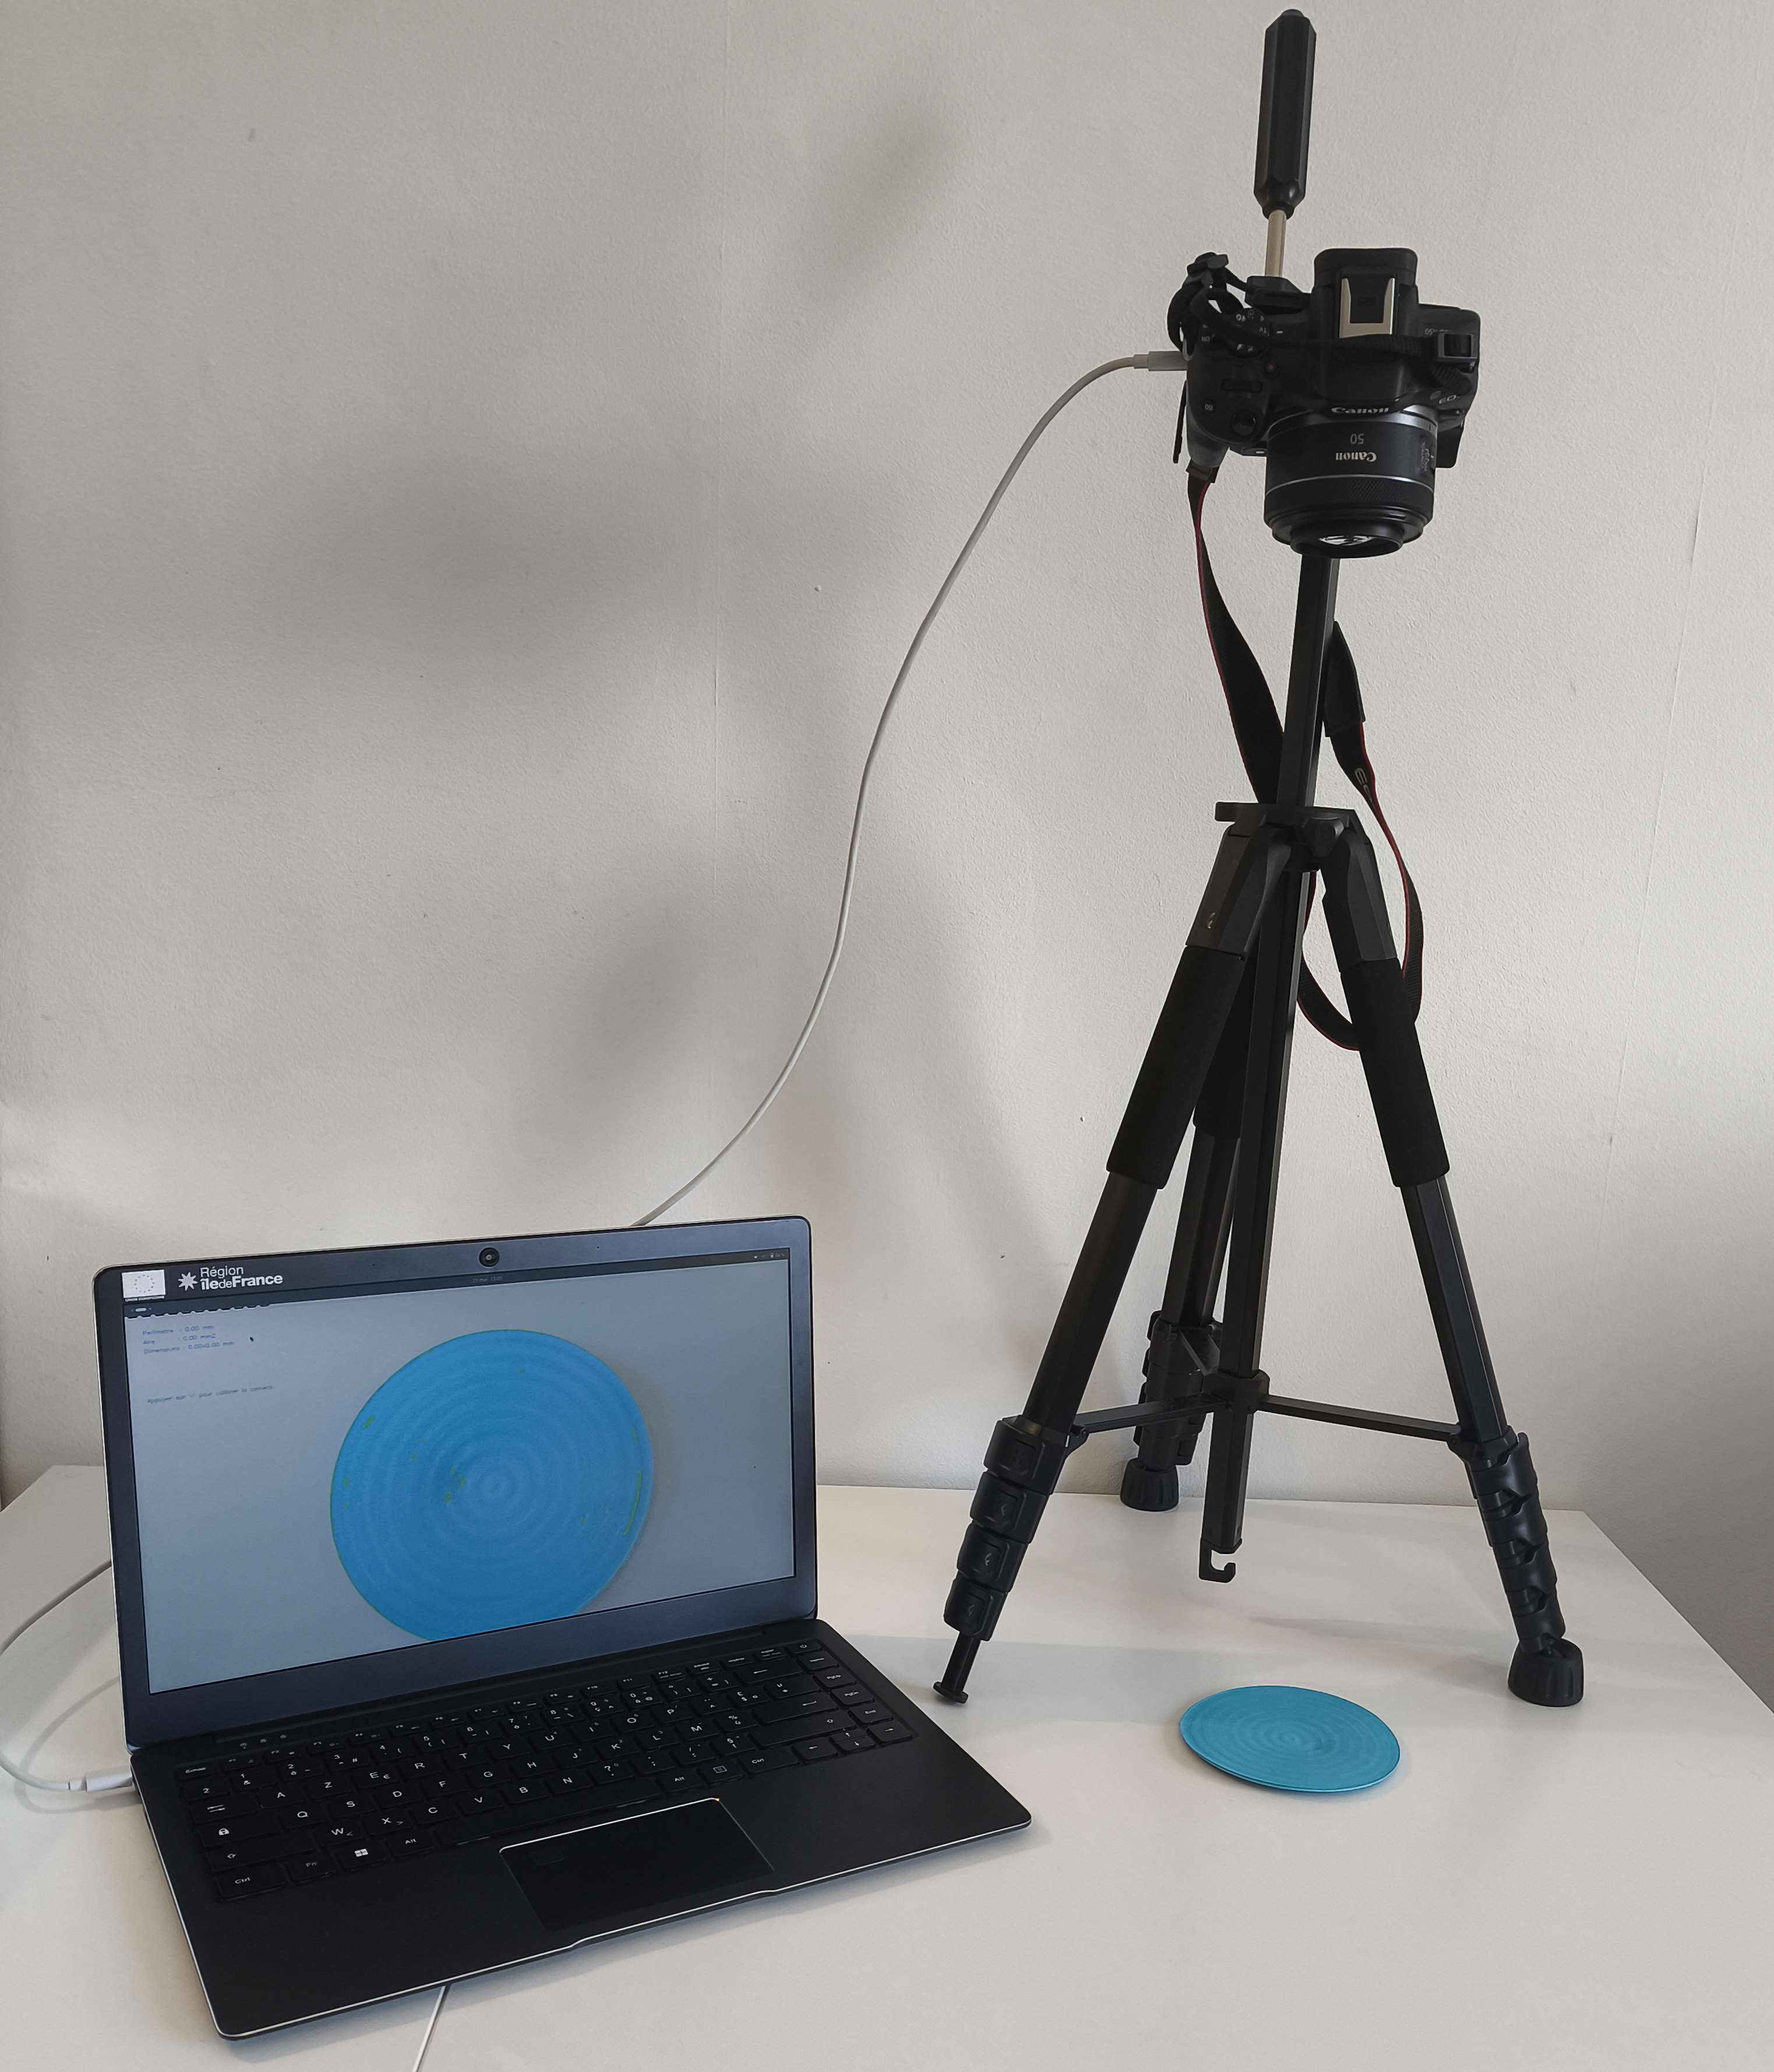
\includegraphics[height=9cm]{Montage.jpg}
	
	\vfill
	\end{titlepage}
	\normalsize
	\tableofcontents
	\clearpage
	\section{Fiche de présentation du projet CPB1}
	\subsection{Étudiants}
	\raggedright\theauthor \\ Année universitaire 2025/2026.
	\subsection{Le rapport de projet }
	Titre du projet : "Métrologie depuis un flux vidéo avec Python."\\[0.5cm]
	Mots clés pour décrire le projet : \\ Python, Mesures, Vidéo \\[0.5cm]
	Court résumé du projet : \\
	Ce projet porte sur la conception d'un système de métrologie en temps réel, capable de mesurer automatiquement le périmètre, la surface et les dimensions d'un objet placé devant une caméra. Le traitement est assuré par un script Python s'appuyant sur la librairie OpenCV, à partir d'un flux vidéo acquis avec un appareil photo positionné à hauteur fixe. Ce système trouve des applications concrètes dans des domaines variés, comme le contrôle qualité en production.\\[0.5cm]
	Court résumé du projet en anglais : \\
	This project focuses on the design of a real-time metrology system, capable of automatically measuring the perimeter, surface area and dimensions of an object placed in front of a camera. The processing is made by a Python script based on the OpenCV library, using a video stream captured with a camera positioned at a fixed height. This system has concrete applications in various fields, such as quality control in production
	
	\clearpage
	\subsection{Formulaire d'informations sur le plagiat }
	Dans le règlement des examens validé par la CFVU de l’UHA, le plagiat est assimilé à une fraude.
	Le plagiat consiste à reproduire un texte, une partie d’un texte, des données ou des images, toute production (texte ou image), ou à paraphraser un texte sans indiquer la provenance ou l’auteur. Le plagiat enfreint les règles de la déontologie universitaire et il constitue une fraude. Le plagiat constitue également une atteinte au droit d’auteur et à la propriété intellectuelle, susceptible d’être assimilé à un délit de contrefaçon.
	En cas de plagiat dans un devoir, dossier, mémoire ou thèse, l’étudiant sera présenté à la section disciplinaire de l’université qui pourra prononcer des sanctions allant de l’avertissement à l’exclusion.
	Dans le cas où le plagiat est aussi caractérisé comme étant une contrefaçon, d’éventuelles poursuites judiciaires pourront s’ajouter à la procédure disciplinaire. \\[0.5cm]
	Je soussigné: \theauthor \\
	Etudiants à l’Université de Haute Alsace en : 2025-2026\\
	Niveau d’études : BAC\\
	Formation ou parcours : CPB1 ENSISA\\
	Reconnaissons avoir pris connaissance du formulaire d’information sur le plagiat.\\
	Fait à Mulhouse 68200\\
	Le 12/05/2026\\
	Signatures :\\
	\includegraphics[width=5cm]{Signature.png}\includegraphics[width=5cm]{Signature_A.png}
	\clearpage
	
	
	\section{Introduction}
	\subsection{Choix du projet}
	Les raisons qui nous ont poussé à choisir ce sujet pour notre projet sont nombreuses. Étant tous les deux passionnés de photographie, nous souhaitions naturellement orienter notre travail autour du traitement d'image. L'idée d'exploiter un flux vidéo en temps réel nous a donc semblé être intéressante, d'autant qu'elle nous permettait de combiner cette passion avec notre intérêt pour la programmation et l'informatique en général.
	
	De plus, nous tenions à proposer un projet qui ait du sens au moment de la présentation. Un programme capable de mesurer automatiquement la surface et le périmètre d'un objet simplement en le plaçant devant une caméra offre un résultat immédiatement visible et compréhensible, ce qui nous paraissait important pour illustrer concrètement notre travail.
	
	Nous avons aussi pensé à l'aspect matériel : ce type de projet ne nécessite pas d'équipement coûteux ou difficile à se procurer. Une caméra standard et un ordinateur suffisent, ce qui rendait le projet accessible et réalisable dans le cadre de notre formation.
	
	Enfin, ce projet ouvre la voie à de nombreuses améliorations futures. La détection de formes, la prise en compte de la perspective, la reconnaissance d'objets spécifiques... les évolutions possibles sont nombreuses.
	\subsection{Description du Projet}
		Ce projet vise à mettre en place un système de métrologie en temps réel grâce à un flux vidéo acquis et traité grâce a python. Nous cherchons donc à pouvoir mesurer des objets placés devant une caméra grâce à y script Python.
	\subsection{Applications}
		\begin{itemize}
			\item 
			
			Ce système peut, par exemple permettre de détecter des objets sur une chaîne de production et de contrôler leur taille afin de mettre en évidence les produits défectueux, sans ralentir la production.
			\item 
			Ce système peut également servir à créer des plans de coupe à l'échelle en mesurant la surface qu'un objet occupe sur l'image.
			\item 
			Nous pouvons également trouver des applications dans la recherche. Nous pouvons prendre comme exemple l'archéologie où les chercheurs classifient souvent les objet découvert par taille. Ce travail de mesure peut être grandement simplifié par des outils de métrologie numériques similaires à notre projet.
		\end{itemize}
	\subsection{Montage expérimental} 
		\begin{itemize}
			\item 
			
			On utilise un appareil photo Canon EOS R50 avec un objectif à focale fixe de 50 mm afin de minimiser les aberrations optiques.
			\item
			On positionne l'appareil sur un trépied réglé à l'aide d'un niveau à bulle de hauteur connue.
			\item
			Le capteur doit être parallèle à la surface sur laquelle l'objet est placé.
			\item
			On utilise un fond uni de couleur différente de celle de l'objet pour faire ressortir l'objet mesuré de l'arrière plan.
			\item
			On connecte la caméra en USB à un ordinateur.
			\item
			Depuis l'ordinateur, on commence l'acquisition.
			
			
		\end{itemize}
	\subsection{Objectifs et contraintes} 
	\raggedright
	À travers ce projet nous voulons récupérer les mesures d'un objet quelconque suivantes : 
		\begin{itemize}
			\item 
			Le périmètre de l'objet.
			\item
			La surface de la face de l'objet montrée à la caméra.
			\item
			Les dimensions de l'objet (longueur et largeur)\\[0.5cm]
		\end{itemize}
	Afin de pouvoir mesurer correctement un objet, nous devons devons définir plusieurs contraintes :
		\begin{itemize}
			\item 
			La calibration de l'appareil permet de convertir des mesures en pixels en millimètres.
			\item 
			Nous devons définir la précision des mesures pour savoir quels objets nous pouvons mesurer correctement.
			\item 
			Nous devons faire des algorithmes de traitement et de calibration d'image.
		
		\end{itemize}
	\section{Code du projet}
	\subsection{Organisation des fichiers}
		Le code de notre projet se compose de quatre fichiers :\\
		\begin{itemize}
			\item 
			Le fichier "main.py" initie et structure notre code. C'est à partir de ce fichier que nous faisons nos mesures.
			\item 
			Le fichier "Traitement.py" contient une fonction traitement prenant en paramètre l'image brut de la caméra et  renvoie un tableau numpy contenant les différents contours de l'objet. 
			\item 
			Le fichier "Mesures.py" contient un ensemble de fonctions qui renvoient les différentes mesures en pixels du plus grand contour que nous trouvons.
			\item 
			Le fichier "Optique.py" contient des fonctions qui renvoient le rapport de pixels par millimètre de l'image nous permettant de convertir nos mesures renvoyées par les fonctions du fichier "Mesures.py" en millimètres.\\[0.5cm]
		\end{itemize}
		\raggedright
		Dans l'ensemble de nos fichiers, nous allons utiliser les librairies OpenCV (cv2) pour la gestion de la caméra et numpy (np) pour la gestion de tableaux (images)
	
	\subsection{Main.py}
	\subsubsection{Problématique}
	Le programme principal constitue le point d'entrée de l'application. Il assure la capture du flux vidéo en temps réel, orchestre les différentes étapes du traitement (calibration, détection des contours, mesure), et affiche les résultats à l'écran. Il repose sur plusieurs modules externes : cv2 pour la capture et l'affichage vidéo, Traitement pour la détection des contours, mesures pour le calcul des grandeurs géométriques, et optique pour la calibration.
	\subsubsection{Principe}
	Le programme principal constitue le point d'entrée de l'application. Il assure la capture du flux vidéo en temps réel, orchestre les différentes étapes du traitement (calibration, détection des contours, mesure), et affiche les résultats à l'écran. Il repose sur plusieurs modules externes : cv2 pour la capture et l'affichage vidéo, Traitement pour la détection des contours, mesures pour le calcul des grandeurs géométriques, et optique pour la calibration.
	\subsubsection{Explication du code.}
	\begin{itemize}
	\item 
	On importe la bibliothèque OpenCV (cv2) ainsi que les trois autres fichiers du projet
	\end{itemize}
	\begin{lstlisting}
	import cv2 
	import Traitement as t
	import mesures as m
	import optique as o
	\end{lstlisting}
	\begin{itemize}
		\item
		On définit les variables de calibration et de mesure ainsi qu'un compteur qui enregistre le nombre de mesures.
		\item
		On définit la variable cap qui va récupérer le flux vidéo de la caméra.
	\end{itemize}
	\begin{lstlisting}
	ratio_px_mm = -1
	ratio_mm_px = -1
	i=0
	perimetre,aire,largeur,hauteur = (0,0,0,0)
	cap= cv2.VideoCapture(0)
	\end{lstlisting}
	\begin{itemize}
		\item
		On initie une boucle infinie dans laquelle on exécute le reste du programme.
		\item
		On définie une variable key qui enregistre la touche du clavier pressée.
		\item
		On définit la variable frame (type numpy.ndarray)qui stocke l'information du flux vidéo dans un tableau de pixels RVB.
		\item
		On définit une variable ret (type booléen) qui renvoie True si cap enregistre un flux vidéo et False sinon.
	\end{itemize}
	\begin{lstlisting}
	while True: 
	
		key = cv2.waitKey(1)
		ret,frame=cap.read()
		
		if not ret: break  
		contours = t.traitement(frame)
	\end{lstlisting}
	\begin{lstlisting}
		if ratio_px_mm == -1:
		
			cv2.putText(frame, "Appuyer sur 'c' pour calibrer la camera",(40, 225),cv2.FONT_HERSHEY_SIMPLEX, 0.5, (255,0,0), 1)
			
			if key == ord("c"):
			
				ratio_px_mm , ratio_mm_px = o.calibration(frame)
	\end{lstlisting}
	\begin{itemize}
		\item 
		On vérifie si le ratio de calibration n'a pas encore été défini (valeur par défaut −1).
		\item
		Si c'est le cas, on affiche un message à l'écran invitant l'utilisateur à appuyer sur 'c' pour calibrer la caméra.
		\item
		Si la touche 'c' est pressée, on appelle la fonction de calibration du fichier optique qui retourne les deux ratios de conversion pixels/mm et mm/pixels.
	\end{itemize}
	\begin{lstlisting}
		else :
			if key & 0xFF == ord(" "):
				
				i+=1
				perimetre,aire,largeur,hauteur = m.mesures(contours)
				print(f"Mesure {i} : \nPerimetre  : {perimetre*ratio_mm_px:.2f} mm\nAire       : {aire*ratio_mm_px**2:.2f} mm2\nDimensions : {largeur*ratio_mm_px:.2f}x{hauteur*ratio_mm_px:.2f} mm")
			cv2.putText(frame, "Appuyer sur espace pour prendre une mesure",(40, 200),cv2.FONT_HERSHEY_SIMPLEX, 0.5, (255,0,0), 1)
	\end{lstlisting}
	\begin{itemize}
		\item
		Une fois la calibration effectuée, on entre dans le bloc else.
		\item
		Si l'utilisateur appuie sur la touche espace, on incrémente le compteur de mesures i, puis on appelle la fonction mesures du fichier mesures qui retourne le périmètre, l'aire, la largeur et la hauteur de l'objet détecté.
		\item
		On affiche ensuite dans le terminal les valeurs converties en millimètres grâce aux ratios calculés lors de la calibration.
		\item
		On affiche également un message à l'écran indiquant à l'utilisateur comment déclencher une mesure.
	\end{itemize}
	\begin{lstlisting}
		cv2.putText(frame, f"Perimetre  : {perimetre*ratio_mm_px:.2f} mm",(40, 40),cv2.FONT_HERSHEY_SIMPLEX, 0.5, (255,0,0), 1)
		cv2.putText(frame, f"Aire       : {aire*ratio_mm_px**2:.2f} mm2",(40, 65),cv2.FONT_HERSHEY_SIMPLEX, 0.5, (255,0,0), 1)
		cv2.putText(frame, f"Dimensions : {largeur*ratio_mm_px:.2f}x{hauteur*ratio_mm_px:.2f} mm",(40, 90),cv2.FONT_HERSHEY_SIMPLEX, 0.5, (255,0,0), 1)
		cv2.imshow('1',frame)   
	
	
		if key & 0xFF == ord('q'): break 
	\end{lstlisting}

	\begin{itemize}
		\item
		Indépendamment de l'état de calibration, on affiche en permanence sur l'image les dernières valeurs de périmètre, d'aire et de dimensions enregistrées, 	converties en millimètres.
		\item
		On affiche la frame courante dans une fenêtre nommée "1".
		\item
		On arrête la boucle si la touche 'q' est pressée.
	\end{itemize}

	\begin{lstlisting}
	cap.release() 
	cv2.destroyAllWindows() 
	\end{lstlisting}
	\begin{itemize}
		\item 
		Une fois la boucle terminée, on libère la caméra afin qu'elle reste accessible pour d'autres programmes.
		\item 
		On ferme toutes les fenêtres ouvertes par OpenCV.
	\end{itemize}
	\subsection{Traitement.py}
	\subsubsection{Problématique.}
	Avant de pouvoir calculer les grandeurs géométriques d'un objet, il est nécessaire d'extraire ses contours à partir de l'image brute capturée par la caméra. Cette étape de traitement d'image repose sur la détection des variations d'intensité lumineuse entre l'objet et son arrière-plan. Ce module regroupe les fonctions nécessaires à cette détection, depuis la conversion de l'image jusqu'à l'extraction des contours.
	
	\subsubsection{Principe.}
	Le traitement s'effectue en plusieurs étapes successives. L'image couleur est d'abord convertie en niveaux de gris pour simplifier les calculs. Un filtre de Sobel est ensuite appliqué pour détecter les contours en identifiant les zones de forte variation d'intensité. L'image résultante est binarisée, puis les contours sont extraits et dessinés sur l'image originale.
	
	\subsubsection{Explication du code.}
	\begin{lstlisting}
	import cv2
	import numpy as np
	import mesures as m
	\end{lstlisting}
	\begin{itemize}
		\item 
		On importe les librairies OpenCV, numpy et le fichier mesures.py
	\end{itemize}
	\begin{lstlisting}
	def Sobel(gray,seuil):
		g = gray.astype(np.float32)
	\end{lstlisting}
	\begin{itemize}
		\item
		On initie la fonction Sobel qui prend en paramètre une image en niveaux de gris et un seuil. Cette fonction renvoie une image binaire grâce a un filtre de 
		Sobel.
		\item 
		On change le type des valeurs contenues dans l'image en niveaux de gris pour avoir des nombres flottants utilisables par numpy. 
	\end{itemize}
	\begin{lstlisting}
		Gx = (  -g[:-2, :-2] + g[:-2, 2:]
			- 2*g[1:-1, :-2] + 2*g[1:-1, 2:]
			-   g[2:,  :-2] + g[2:,  2:] )
		Gy = (  -g[:-2, :-2] - 2*g[:-2, 1:-1] - g[:-2, 2:]
			+  g[2:,  :-2] + 2*g[2:,  1:-1] + g[2:,  2:] )
	\end{lstlisting}
	\begin{itemize}
		
		\item On Calcule le gradient horizontal en appliquant le noyau Sobel $K_x$ par slicing vectorisé, détecte les contours verticaux.
		
		\item On Calcule le gradient vertical en appliquant le noyau Sobel $K_y$ par slicing vectorisé, détecte les contours horizontaux.
		
	\end{itemize}
	\begin{lstlisting}
		G = np.sqrt(Gx**2+Gy**2)
		G = (G / G.max() * 255).astype(np.uint8)
	
		binary = (G > seuil).astype(np.uint8) * 255
	
		return binary
		
	\end{lstlisting}
	\begin{itemize}
		\item On Calcule la magnitude du gradient en combinant $G_x$ et $G_y$ via la norme euclidienne.
		
		\item On Normalise les valeurs dans l'intervalle $[0, 255]$ et reconvertit en entiers 8 bits.
		
		\item On Applique le seuil : chaque pixel devient 255 si c'est un contour détecté, 0 sinon.
		
		\item On renvoie l'image binaire des contours détectés.
	\end{itemize}
	\begin{lstlisting}
	def traitement(frame):
		
		gray = cv2.cvtColor(frame, cv2.COLOR_BGR2GRAY)
		binary = Sobel(gray, 50)
		contours, _ = cv2.findContours(binary, cv2.RETR_EXTERNAL, cv2.CHAIN_APPROX_SIMPLE)
		cv2.drawContours(frame, contours,-1,(0,255,0))
		return contours
	\end{lstlisting}
	\begin{itemize}
		\item
		On initie une fonction traitement qui prend en paramètre l'image brute transmise par la caméra.
		\item 
		On passe l'image (espace de couleur sRGB) en niveau de gris pour pouvoir la passer en image binaire
		\item
		On utilise notre filtre de Sobel pour obtenir une image binaire 
		\item 
		À partir de l'image binaire on obtient une liste de contours grâce a la fonction cv2.findContours.
		\item
		On dessine les contours en vert sur l'image initiale pour les visualiser.
		\item
		On renvoies la liste de contours pour pouvoir l'exploiter.
	\end{itemize}
	\subsection{Mesures.py}
	\subsubsection{Problématique}
	Une fois les contours de l'objet détectés dans l'image, il est nécessaire d'en extraire des grandeurs géométriques exploitables : le périmètre, l'aire, et les dimensions (largeur et hauteur). Ces grandeurs sont d'abord calculées en pixels, puis converties en millimètres par le programme principal à l'aide du ratio de calibration. Ce module regroupe l'ensemble des fonctions nécessaires à ces calculs.
	
	\subsubsection{Principe}
	Le module s'appuie sur la bibliothèque numpy pour effectuer des calculs vectoriels efficaces sur les coordonnées des points du contour, ainsi que sur numba pour accélérer la fonction la plus coûteuse en calcul. Chaque grandeur géométrique est calculée par une fonction dédiée, et une fonction principale mesures() orchestre l'ensemble en sélectionnant le contour le plus pertinent et en retournant toutes les grandeurs en une seule fois.
	\subsubsection{Explication du code.}
	\begin{itemize}
		\item
		On importe la bibliothèque numpy pour pouvoir travailler sur les contours de type numpy.ndarray.
		\item 
		On importe la bibliothèque numba pour compiler certains algorithmes trop lourds.
	\end{itemize}
	\begin{lstlisting}
	import numpy as np
	from numba import njit
	\end{lstlisting}
	\textbf{}{Calcul du périmètre de l'objet.}
	\begin{lstlisting}
	def perimetre(contour):    
		pts = contour.reshape(-1, 2)
		diff = pts - np.roll(pts, -1, axis=0)
		distances = np.sqrt((diff**2).sum(axis=1))
		p = distances.sum()
		return p
	\end{lstlisting}
	\begin{itemize}
	\item On crée un tableau de points à partir du contour. On utilise la méthode .reshape pour changer la forme du contour de (Nombre de points,1,Coordonnées du point) à (Nombre de points, Coordonnées du point) car OpenCV ajoute une dimension parasite (1) lorsque l'on utilise la fonction cv2.findContours.
	\item 
	On calcule la différence entre tous les points successifs. Pour cela, on soustrait la liste pts décalée de un point par la méthode np.roll à la liste de  pts. On obtient donc une liste de la forme (Nombre de points, ($x_{i} - x_{i+1}$,$y_i - y_{i+1}$).
	\item 
	On calcule ensuite le périmètre en faisant la somme des distances entre les points avec la formule : $$\sum\limits_{i=0}^{n-1}\sqrt{(x_i -x_{i+1})^2+(y_i -y_{i+1})^2}$$ \\
	La méthode .sum(axis=1) fait la somme des coordonnées ($(x_{i} - x_{i+1})^2$,$(y_i - y_{i+1})^2$). Puis np.sqrt calcule la racine de cette somme pour chaque point de diff**2.
	\item 
	On initie la variable p qui fait la somme de tous les éléments du tableau distances. 
	\item 
	La fonction renvoie la variable p qui correspond au périmètre.
	
	
	\end{itemize}
	\textbf{Calcul de l'aire de l'objet.}
	\begin{lstlisting}
	def aire(contour):  
		pts = contour.reshape(-1, 2)
		x = pts[:, 0]
		y = pts[:, 1]
		a = 0.5 * abs(np.dot(x, np.roll(y, -1)) - np.dot(y, np.roll(x, -1)))
		return a
	\end{lstlisting}
	\begin{itemize}
		\item 
		On crée un tableau pts à partir du tableau contour dont la forme a été modifiée avec la méthode .reshape.
		\item 
		
	\end{itemize}
	\textbf{Calcul des dimensions de l'objet.}
	\begin{lstlisting}
	@njit
	def dimensions(contour):
		pts = contour.reshape(-1, 2).astype(np.float64)
	
		x_min = np.min(pts[:, 0])
		y_min = np.min(pts[:, 1])
		
		x_max = np.max(pts[:, 0])
		y_max = np.max(pts[:, 1])
	\end{lstlisting}
	\begin{itemize}
		\item
		On utilise le décorateur njit de la librairie numba pour compiler la fonction avant l'exécution du programme pour l'accélérer.
		\item 
		On initialise la fonction dimensions qui prend en paramètre un seul contour.
		\item 
		On crée un tableau pts à partir du tableau contour dont la forme a été modifiée avec la méthode .reshape.
		\item 
		On cherche les points avec les coordonnées $(x_{min},y_{min})$ minimales et $(x_{max},y_{max})$ maximales. Pour cela, on utilise les fonctions np.min() et np.max() qui parcourent tous les points du tableau afin de renvoyer respectivement les valeurs des coordonnées minimales et maximale du tableau de points.
	\end{itemize}
	\begin{lstlisting}
		aire = (x_max - x_min) * (y_max - y_min)
		dims = (x_max - x_min, y_max - y_min)
	\end{lstlisting}
	\begin{itemize}
		\item On définit l'aire formée par le rectangle encadrant l'objet par : $$Aire =(x_{max} - x_{min}) * (y_{max} - y_{min}) $$
		\item
		On stocke la hauteur et la largeur de ce rectangle dans un tuple dims 
	\end{itemize}
	\begin{lstlisting}
		rad = np.pi / 180
		c = np.cos(rad)
		s = np.sin(rad)
	\end{lstlisting}
	\begin{itemize}
		\item On définit la fonction cosinus, sinus ainsi que la valeur d'un radiant.
	\end{itemize}
	\begin{lstlisting}
		
		for _ in range(360):
			for i in range(len(pts)):
				x, y = pts[i]
				pts[i][0] = x * c - y * s
				pts[i][1] = x * s + y * c
	\end{lstlisting}
	\begin{itemize}
		\item 
		Afin d'obtenir la longueur et la largeur de l'objet, nous devons le tourner sur 360 pour trouver l'angle où l'objet est est encadré par le plus petit rectangle possible.
		\item 
		On tourne l'objet de 1° 360 fois et pour chaque points, on modifie les coordonnées suivant les formules suivantes : $$x_{final} = x_{initial}*cos(1°)-y_{initial}*sin(1°)$$ $$y_{final} = x_{initial}*sin(1°)+y_{initial}*cos(1°)$$
	\end{itemize}
	\begin{lstlisting}	
		
			x_min = np.min(pts[:, 0])
			y_min = np.min(pts[:, 1])
			
			x_max = np.max(pts[:, 0])
			y_max = np.max(pts[:, 1])
	
			largeur = x_max - x_min
			hauteur = y_max - y_min
			aire2 = largeur * hauteur
	\end{lstlisting}
	\begin{itemize}
	\item 
	On redéfinit les points avec les coordonnées minimales et maximales de l'image tournée.
	\item 
	On définit la largeur et la hauteur du nouveau rectangle encadrant l'objet
	\item 
	On calcule l'aire de ce rectangle.
	
	\end{itemize}
	\begin{lstlisting}
	
			if aire2 < aire:
				aire = aire2
				dims = (largeur, hauteur)
	
		return dims
	\end{lstlisting}
	\begin{itemize}
		\item On compare l'aire du nouveau rectangle (aire2) avec la valeur stockée dans la variable aire.
		\item Si l'aire du nouveau rectangle est inférieur à celle du précédent, alors on remplace la valeur stockée dans la variable aire par celle de aire2 et on remplace les valeurs stockée dans la variable dims par les dimensions du nouveau rectangle.
		\item lorsque tous les angles ont été testés, on renvoie la variable dims.
	\end{itemize}
	\textbf{Fonction mesure(contours).}
	\begin{lstlisting}
	def mesures(contours):
		contour=max(contours, key=perimetre)
		p = perimetre(contour)
		a = aire(contour)
		d = dimensions(contour)
		return float(p),float(a),float(d[0]),float(d[1])
	\end{lstlisting}
	\begin{itemize}
		\item On définit une fonction mesures qui prend en paramètre l'ensemble des contours renvoyés par la fonction cv2.findContours.
		\item On stocke le plus grand contour de la liste dans le tableau contour. Ce contour est choisi en comparant les contours par leur image de la fonction périmètre
	\end{itemize}
		
	\subsection{Optique.py}
	\subsubsection{Problématique.}
	Les mesures brutes extraites de l'image par traitement vidéo sont exprimées en pixels. Or, pour obtenir des grandeurs physiques exploitables (surface en mm², périmètre en mm), il est nécessaire de connaître la correspondance entre un pixel et une distance réelle en millimètres. Cette correspondance dépend de la distance entre l'objet et la caméra, ainsi que des paramètres optiques de celle-ci. Une étape de calibration est donc indispensable avant toute mesure.
	\subsubsection{Principe.}
	La méthode retenue repose sur l'utilisation d'un objet de calibration de dimensions connues. On vient placer cet objet devant la caméra à la distance de travail souhaitée, puis donne sa longueur réelle en millimètres. Le programme détecte automatiquement le contour de cet objet dans l'image et en mesure la dimension en pixels. Le rapport entre ces deux grandeurs fournit le ratio de conversion. Deux ratios sont calculés et retournés : le ratio\_px\_par\_mm, qui indique le nombre de pixels correspondant à 1 mm, et le ratio\_mm\_par:\_px, qui indique le nombre de millimètres correspondant à 1 pixel et qui sera utilisé pour les mesures.
	\subsubsection{Explication du code.}
	\begin{lstlisting}
		import cv2 
		import numpy as np
		import Traitement as t 
		import mesures as m
	\end{lstlisting}
	\begin{itemize}
		\item
		On importe les librairies numpy, OpenCV ainsi que les fichiers Traitements.py et mesures.py
	\end{itemize}
	\begin{lstlisting}
		def calibration(contours):
			flottant =  False
			while flottant is not True :
				try :
					longueur_reele_mm = float(input("Longueur reelle de l'objet de calibration (mm) : "))
					flottant = True
				except : 
					flottant = False 
	\end{lstlisting}
	\begin{itemize}
		\item
		La fonction calibration(contours) reçoit en paramètre une liste de contours déjà détectés et transmise par le programme appelant.
		\item
		On demande ensuite via une saisie sécurisée la longueur réelle de l'objet utilisé pour la calibration.
	\end{itemize}
	\begin{lstlisting}
			if not contours:
				print("Aucun contour détecté")
				return -1, -1
	\end{lstlisting}
	\begin{itemize}
		\item On vérifie que la fonction ne reçoit pas une variable 'None' en paramètres. Si c'est le cas, la fonction renvoie (-1,-1).
	\end{itemize}
	\begin{lstlisting}
			contour = max(contours, key=lambda c: m.aire(c))
	\end{lstlisting}
	\begin{itemize}
		\item On cherche à récupérer le plus grand contour. Pour cela, on parcourt la liste de contours via la variable c. Chaque contour est comparé selon son aire calculée par la fonction m.aire(c). Le contour avec l'aire la plus grande est ensuite stockée dans le tableau contour.
	\end{itemize}
	\begin{lstlisting}
			largeur_px, hauteur_px = m.dimensions(contour)
			longueur_px = max(largeur_px, hauteur_px)
	\end{lstlisting}
	\begin{itemize}
		\item On récupère la largeur et la hauteur de l'objet de calibration grâce a la fonction m.dimension(contour)
		\item
		On recherche la plus grande des deux dimensions renvoyés que l'on stocke dans variable longueur\_px.
	\end{itemize}
	\begin{lstlisting}
			ratio_px_par_mm = longueur_px / longueur_reele_mm
			ratio_mm_par_px = longueur_reele_mm / longueur_px
		
			print(f"Longueur en pixels : {longueur_px:.1f} px")
			print(f"Ratio : {ratio_px_par_mm:.3f} px/mm")
		
			return float(ratio_px_par_mm), float(ratio_mm_par_px)
	\end{lstlisting}
	\begin{itemize}
		\item
		Les deux ratios de conversion sont ensuite calculés par une division.
		\item 
		Ces deux valeurs sont affichées dans la console, ce qui permet à l'utilisateur de vérifier la cohérence de la calibration.
		\item 
		Les deux ratio sont renvoyés sous forme de flottants pour être utilisées dans la suite du programme.
		
	\end{itemize}
	\section{Résultats expérimentaux.}
	\subsection{Mesures}
	Nous avons calibré notre caméra avec un disque de 10 cm de diamètre
	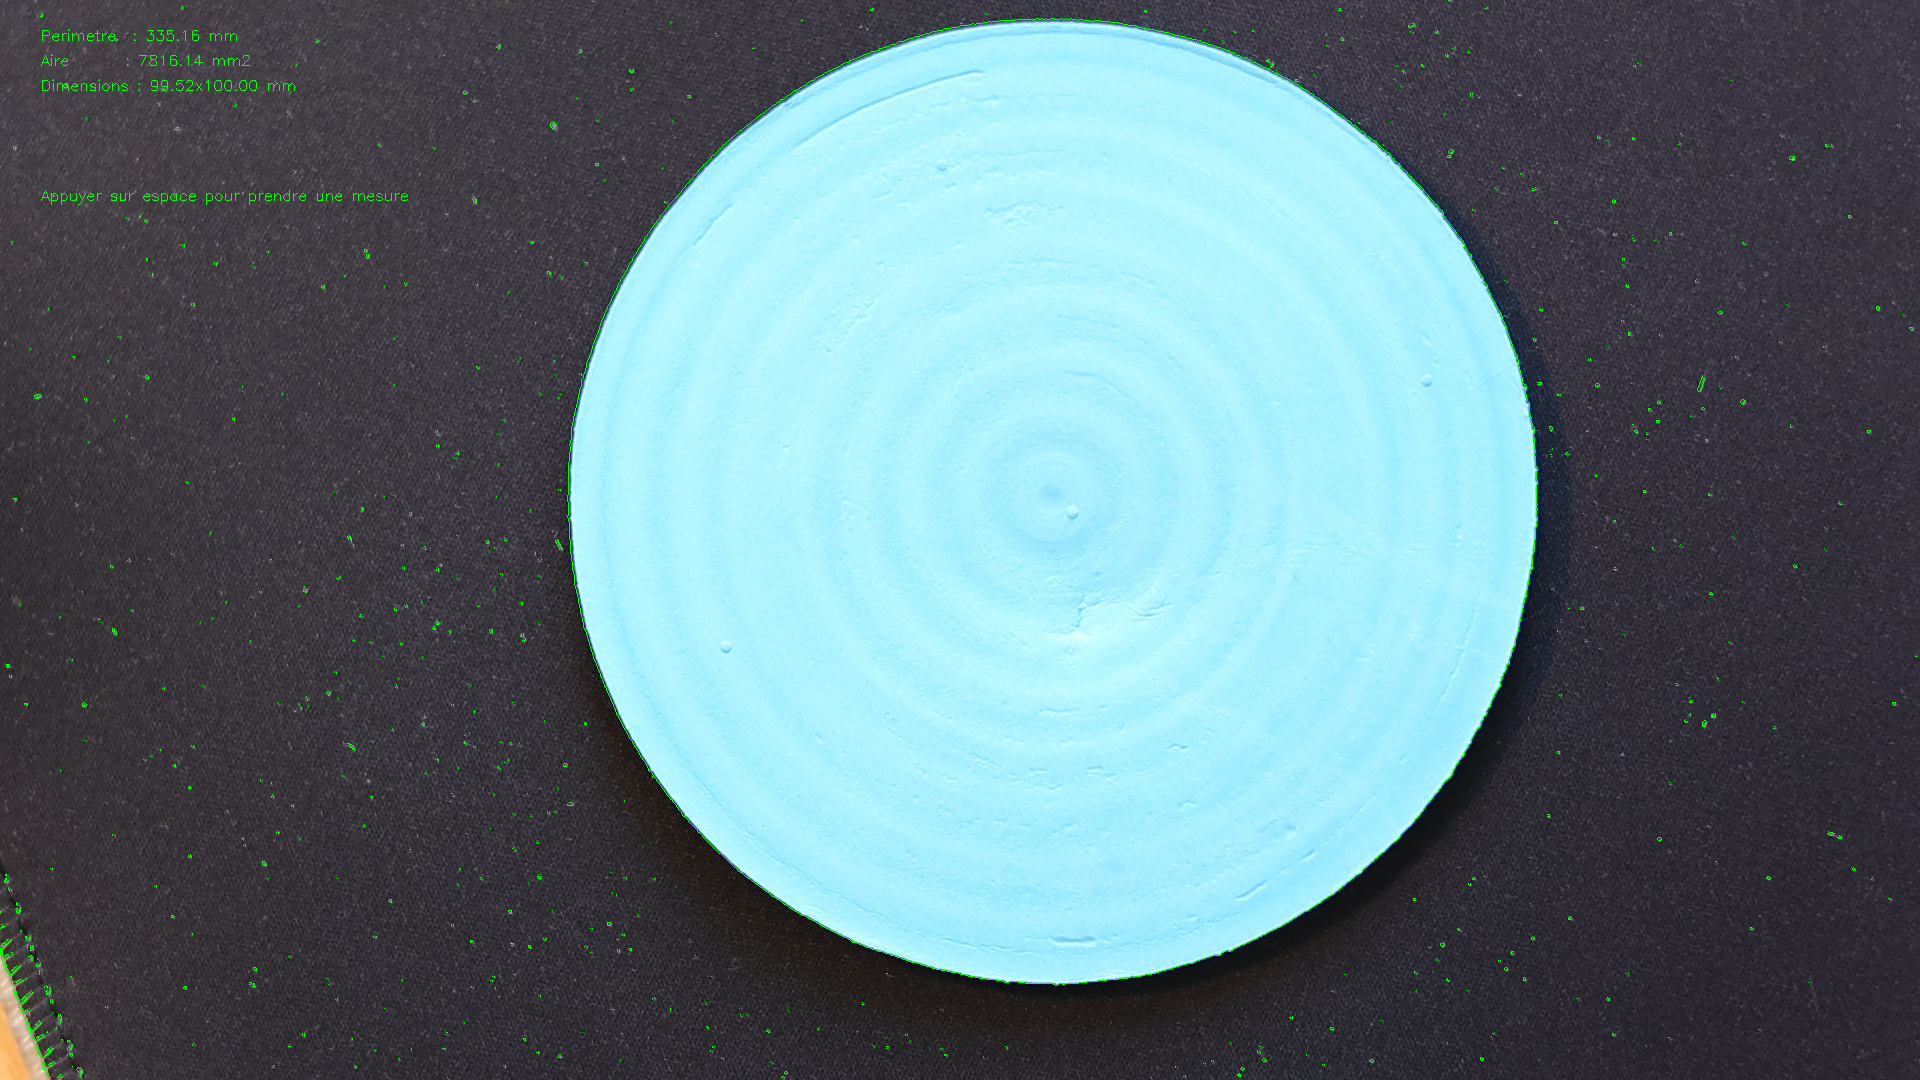
\includegraphics[width=15cm]{Calibration.png}
	Nous pouvons remarquer qu'après les mesures, les résultats sont proches des valeurs théoriques.
	\begin{itemize}
		\item Pour le cas du périmètre, nous avons:
		$$P_{exp} = 335.18 mm et P_{th} = 2* \pi * 50 = 314.16mm$$
		\item pour l'aire , nous avons :
		$$A_{exp} = 7816.14mm^2 et A_{th}= \pi * 50^2 = 7853.98mm$$
	\end{itemize}
	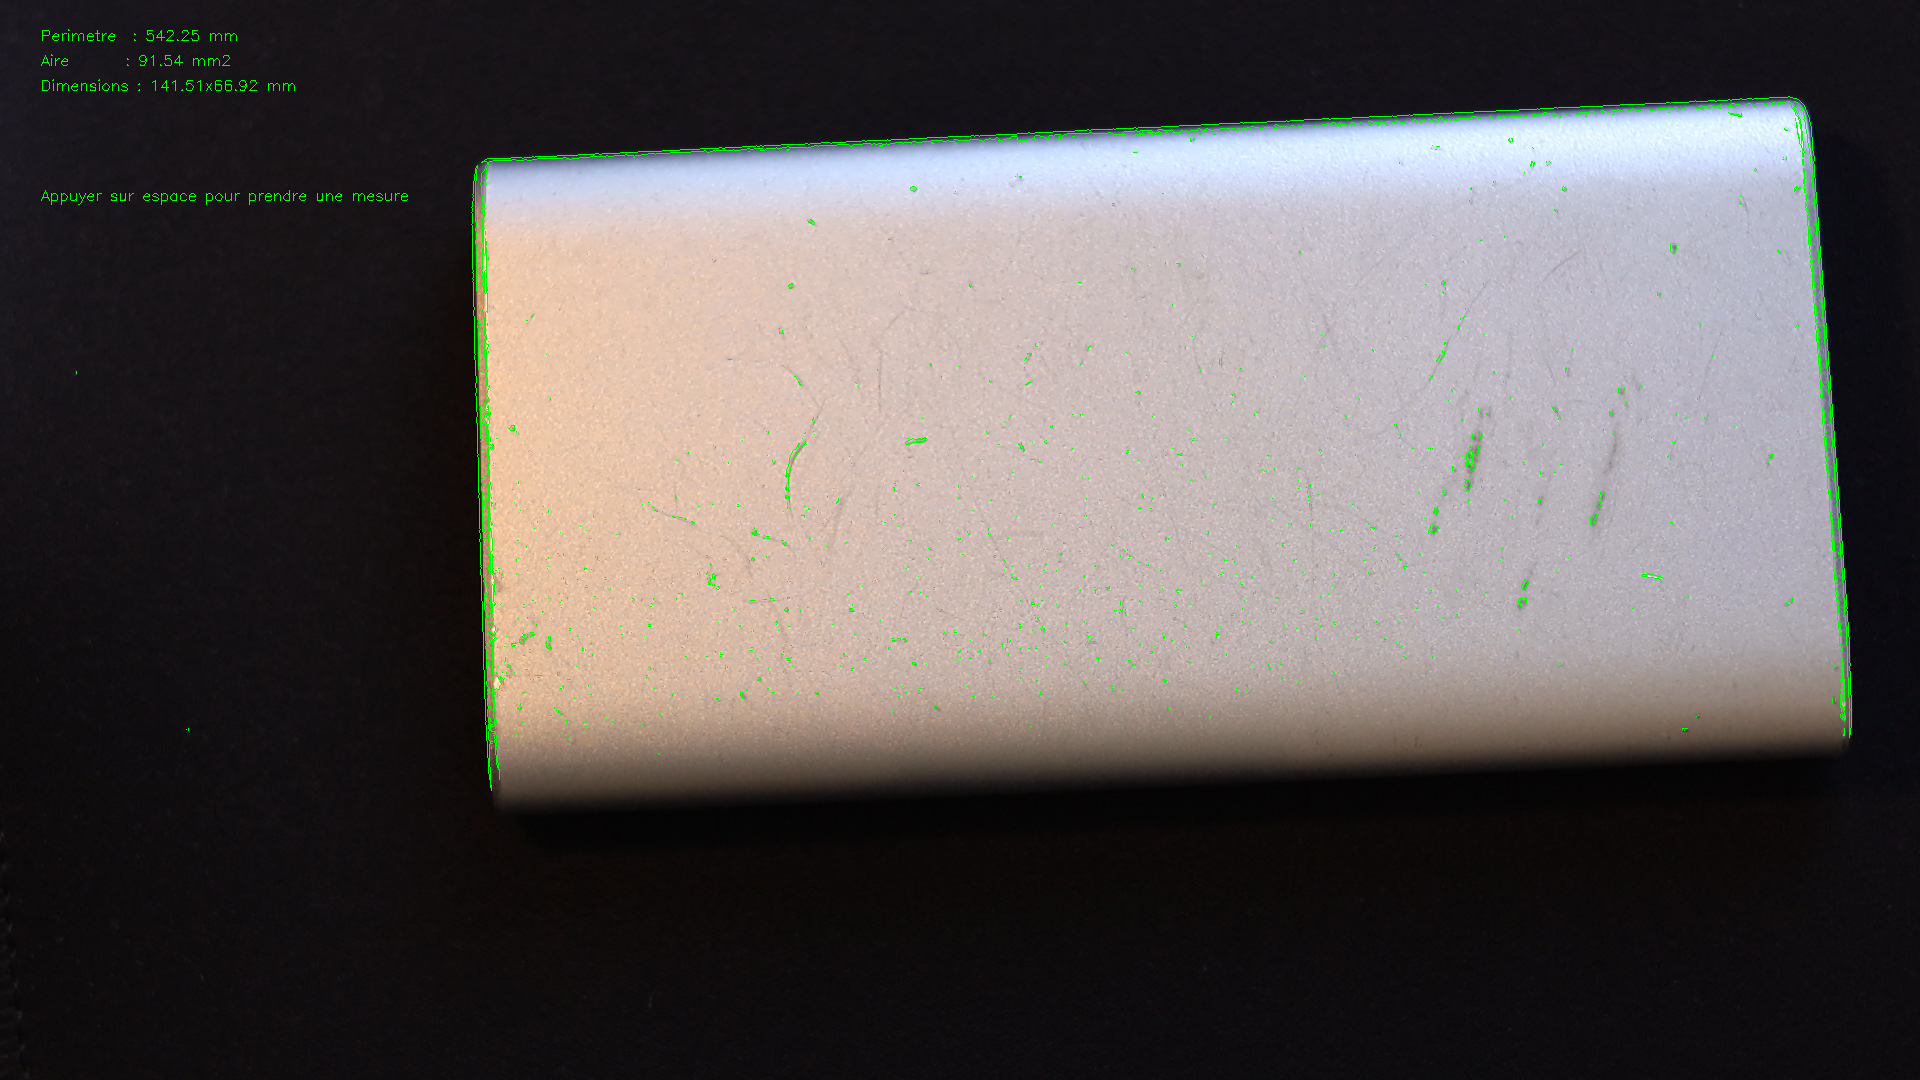
\includegraphics[width=15cm]{Calibration2.png}
	Cependant pour des objets ayant un contour que le logiciel ne capte pas comme fermé, l'aire et le périmètre ont des valeurs aberrantes. Seuls les dimensions correspondent à la taille réelle de l'objet.
	\section{Limites du projet}
	La réalisation de ce projet nous a confrontés à plusieurs difficultés techniques. La première a concerné la calibration : notre première version du code retournait des valeurs incohérentes, ce qui nous a contraints à revoir quasi entièrement ce dernier pour obtenir des ratios de conversion fiables. La deuxième difficulté était liée aux performances : le programme était initialement trop demandant en calcul, ce qui entraînait une chute importante du nombre d'images par seconde et rendait l'utilisation en temps réel difficile. Pour y remédier, nous avons eu recours à la bibliothèque numba, qui permet de compiler certaines fonctions critiques à la volée en code machine, réduisant significativement le temps de calcul.
	
	Dans son état actuel, le projet est loin d’être parfait. En effet, ce dernier présente plusieurs limites qu’ils semblent importants de souligner. La première concerne la précision de la détection des contours : le filtre de Sobel est très sensible aux conditions d'éclairage et au contraste entre l'objet et son arrière-plan. Un éclairage inégal ou des reflets peuvent ainsi conduire à une détection incomplète ou imprécise contours, et donc à des mesures fausses. La deuxième limite concerne la calibration : celle-ci est valable uniquement pour une distance entre la caméra et objet fixe, et doit être recommencée dès que cette distance change. Le programme ne gère pas non plus les distorsions optiques et géométrique de la caméra, qui peuvent introduire des erreurs de mesure, notamment sur les bords de l'image. La troisième limite porte sur le calcul des dimensions : la méthode du rectangle englobant minimal par rotation exhaustive degré par degré introduit une imprécision angulaire pouvant légèrement fausser les dimensions retournées. Enfin, le programme ne gère qu'un seul objet à la fois, en sélectionnant systématiquement le contour le plus grand détecté dans l'image, ce qui le rend inadapté à une utilisation impliquant plusieurs objets simultanément.
	
	\section{Conclusion}
	Ce projet nous a permis de concevoir et de réaliser un système de métrologie en temps réel, capable de mesurer automatiquement le périmètre, la surface et les dimensions d'un objet à partir d'un simple flux vidéo. Les résultats expérimentaux obtenus sont encourageants : pour un disque de 50 mm de rayon, l'erreur relative sur l'aire est inférieure à 0,5\%, ce qui démontre la viabilité de l'approche retenue.
	
	Au-delà des résultats techniques, ce projet nous a apporté beaucoup sur le plan personnel. Nous avons appris à structurer un projet de programmation en plusieurs modules indépendants, à utiliser des bibliothèques scientifiques comme OpenCV, numpy et numba, et à confronter nos résultats à des valeurs théoriques pour valider notre travail. Nous avons également pris conscience de l'importance de l'étape de calibration dans tout système de mesure physique.
	
	Plusieurs améliorations pourraient être envisagées pour faire évoluer ce projet. La correction des distorsions optiques par une calibration de la caméra plus poussée permettrait d'améliorer la précision des mesures, notamment en bords d'image. Enfin, l'extension du programme à la détection et à la mesure simultanée de plusieurs objets ouvrirait la voie à des applications industrielles plus complètes.
\section{Bibliographie.}
\subsection{Cours}
\begin{itemize}
	\item Convolution de matrices (exo7)
	\href{https://exo7math.github.io/deepmath-exo7/convolution2d/convolution2d.pdf}{lien}
	\item Filtrage et détection de contours (Florent Lafarge, INRIA) : \href{https://www-sop.inria.fr/members/Florent.Lafarge/cours/ENS_course_2.pdf}{lien}
	\item Détection de contours, filtre de Sobel et différences de gaussiennes (Caroline Petitjean, Université de Rouen) : \href{http://carolinepetitjean.free.fr/enseignements/ti/cours3_M1_Petitjean.pdf}{lien}
\end{itemize}

\subsection{Articles et tutoriels}
\begin{itemize}
	\item Implémentation du filtre de Sobel en Python (YouTube) : \href{https://www.youtube.com/watch?v=8ugtP_8jri4}{lien}
	\item Détection de contours avec cv2.findContours et cv2.drawContours (LearnOpenCV) : \href{https://learnopencv.com/contour-detection-using-opencv-python-c/}{lien}
	\item Mesure de la taille d'un objet avec OpenCV en Python (GeeksforGeeks) : \href{https://www.geeksforgeeks.org/python/measure-size-of-an-object-using-python-opencv/}{lien}
	\item Projet open-source de mesure d'objets en temps réel avec OpenCV (GitHub) : \href{https://github.com/mishrakushal/real-time-object-measurement}{lien}
\end{itemize}
\end{document}
